

\chapter{Type I Prediction: Structural Modeling}\label{ch:predictor_t1}

\section{Introduction}

% \begin{quote}
% \noindent
% The state of a structure as it experiences an event is assumed to be characterized by its displacement $\displ$ and velocity $\veloc$, which is governed by Newton's laws of motion:
% \begin{equation}
%     \Mass \accel = \extern -  \intern(\displ,\veloc), %\force (\displ, \veloc, \accel) = \mathbf{f}
%     \label{eq:newton-discrete}
% \end{equation}
% where $\accel$ is the acceleration associated with the state of the structure, $\intern$ characterizes the internal resisting force produced by the structure in response to its configuration, and $\extern$ is the external loading that is imposed by the event. \glspl{predictor-t1} are premised on the idea that if the form of $\intern$ is \emph{assumed} and the loading $\extern$ is \emph{given}, then $\displ$ and $\veloc$ can be approximately \emph{determined} by methods of integration of the second order system of differential equations in \cref{eq:newton-discrete}.
% %
% On the \gls{platform}, this is realized by employing a \emph{finite element} approximation of $\Mass$ and $\intern$ and constructing an approximation to $\extern$ from the sensor data.
% \end{quote}

\noindent
In the field of civil engineering, the most ubiquitous class of prediction techniques is those that leverage a structural analysis model.
These techniques are readily
accessible to the large workforce of civil engineers that routinely develops models of
this type for applications in design and rehabilitation.
Structural analysis models are constructed by characterizing the properties of each structural component of an asset. 
Currently,  models of this type that are employed on the \BRACE{} platform leverage advanced finite elements that are typically not available through basic commercial products. 

% For each structure that has its recorded acceleration responses streamed to the \gls{platform}, the platform is able to host a family of structural analysis models that perform response prediction in near real-time. 
% Over time, the growing collection of response predictions can be studied to identify the configurations that are best for generating meaningful condition assessments depending on situational characteristics and requirements (for example, event intensity, prediction resolution and fidelity, and relative modeling costs). From these studies, best practices in structural analysis modeling for health monitoring can be defined; meanwhile, techniques that are more established within the discipline of structural health monitoring tend to fall under the category of ``data-driven" methods.


\Glspl{predictor-t1} can be divided into
\emph{local}, or \emph{component} models, and \emph{global}, or \emph{structure} models. 


\section{Modeling}
\label{sec:chap4_modeling}
%
%
Several models are developed for each bridge with varying fidelities to
target a wide range of events.
In order to accurately represent the structural response to a broad range of
excitation intensities, several \glspl{predictor-t1} may be required. 
For events of low to moderate intensity, a low-fidelity linear model, e.g., \cref{fig:meloland-abut}, often suffices. 
However, in order to compute damage indicators following high intensity events, a high-fidelity nonlinear model is required that is able to account for and report on inelastic and geometrically nonlinear response. 
Because these nonlinear models tend to be computationally intensive, a lower-fidelity model may be utilized to report partial metrics pending the completion of the full nonlinear analysis.
\begin{figure}[H]
\hypertarget{fig:meloland-abuts}{%
\centering
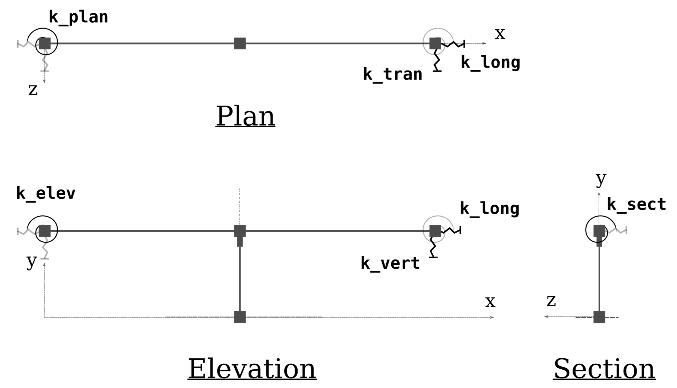
\includegraphics{Part II/figures/meloland/structure-dwg-abuts-new.pdf}
\caption{A low-fidelity model of Caltrans bridge No. \texttt{58-0215} (Meloland Road Overpass).}\label{fig:meloland-abut}
}
\end{figure}

\subsection{Low Fidelity Models}

% \subsubsection{Low-Fidelity Models}
A low-fidelity model may be used to explore and validate the behavior of
an idealized structure in the absence of 
structural degradation such as cracking and creep.
Mass is generally assigned to the structure using consistent mass distribution in all involved frame elements.
%
%
\subsubsection*{Superstructure}

\begin{figure}[H]
\hypertarget{fig:meloland-girder-fe-mesh}{%
\centering
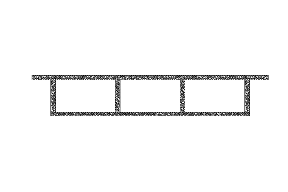
\includegraphics[width=0.5\textwidth, trim = 0 35 0 35, clip]{Part II/figures/meloland-girder-mesh.pdf}
\caption{Finite element model used to obtain the warping constant for the superstructure of Caltrans Bridge No. \texttt{58-0215} Caltrans (Meloland Road Overpass).}\label{fig:meloland-girder-fe-mesh}
}
\end{figure}

In a low-fidelity model, the superstructure is generally modeled using the linear-elastic Euler-Bernoulli
beam model. 
Parameters of this model (i.e., the moment of inertia, cross-sectional area, and elastic modulus) are taken as those of the gross
concrete section, neglecting reinforcement. 
The girder may be assumed homogeneous and details like reduced-strength concrete specified for the deck need not be accounted for \citep{caltrans2019seismic}. 
An independent planar finite element model may be required to calculate the torsion constant of the superstructure girders (see, e.g., \cref{fig:meloland-girder-fe-mesh}).
%
%
Similarly, cap beams are generally modeled as elastic beam-column elements with moment of inertia incorporating an additional flange where the superstructure coincides with the cap beam.
%
%
%
\subsubsection*{Substructure}
A low-fidelity bent model may similarly employ linear-elastic columns with
linear geometry. 
The elements are joined to the superstructure at the centroid of the girder, and a rigid offset is
imposed at this joint with a length equal to the vertical distance
between the centroid and the soffit of the girder.
For some structures, it may be sufficient to impose fixed displacement boundary conditions at the base of the column, but this decision should be made judiciously. 
More sophisticated soil/foundation modeling like those described in \cref{sec:m2-SSI} may be required for certain structures even at the low-fidelity level.
Cap beams are modeled as elastic beam elements with cross-section properties computed from the geometry. 

\subsubsection*{Abutments}
% A simple abutment model may consist of a collection of parameterized linear springs.
In simple overpass structures, special care should be considered in modeling the abutment response, even at the low-fidelity level.
In a study of Caltrans bridge No. \texttt{58-0215} (Meloland Road Overpass), \cite{werner1987seismic} concluded that the abutments and embankments
are the primary contributors to the transverse response, meanwhile
vertical response characteristics were dominated by properties of the
deck.
\textcite{levine1989dynamic} build on the study of
\cite{werner1987seismic} to produce an estimate for linear
rotational stiffnesses at the abutments using a system identification
procedure developed by \textcite{beck1978determining} . 
The model used in this study
is a simple linear 3D beam assemblage with fixed translational
boundary conditions at the abutments.
\textcite{wilson1990bridge} used a \emph{single-input, single-output} (SISO)
structural identification technique to further explore the abutment
response.

\textcite{goel1997evaluation} considered another Caltrans bridge No. \texttt{04-0236} (Painter Street Overcrossing) 
and note that the linear elastic models proposed in the
aforementioned publications are insufficient as they fail to account for
reductions in the abutment stiffness values that arise under the influence of
earthquake motions. This study also evaluated procedures from
Caltrans, AASHTO-83, and ATC-6. 
In another study, 
\textcite{zhang2002seismic} built upon the work of
\textcite{wilson1990bridge}, \cite{werner1987seismic}, and
\textcite{goel1997evaluation}.
%
Finally, \textcite{arici2003system} reviewed most of the aforementioned studies
and sought, among several tasks, to examine the predictive capabilities
of identified linear models using a \emph{multi-input, single-output} (MISO)
 approach.
%
%
%
\subsection{High-Fidelity Models}
A high-fidelity model is able to provide more useful metrics to the \gls{platform}, such as the component damage state card at the top left corner of \cref{fig:SS3}. However, this requires careful
consideration of the inelastic material response throughout the
 structure. 
Material properties such as constitutive relationships of the concrete and the reinforcing steel are determined from common engineering practice and/or testing for the materials used in the structure's construction. 
Generally, these materials include unconfined concrete, confined concrete, steel for reinforcing bars, and elastomers for bearings. They may also include advanced materials such as Fiber Reinforced Polymers (FRP) using carbon or glass fibers for retrofitted structures.

\subsubsection{Columns}
Because bridge damage states often include flexural yielding (plastic hinging) and failures at the columns, it is important that a high-fidelity column model is capable of accurately reporting this inelastic behavior. 
To this end, frame elements that are expected to exhibit inelasticity should be modeled by inelastic elements capable of exhibiting hysteresis. 
For this purpose, a \emph{fiber section} may be used to collocate material points over the cross-section. 
Accordingly, uniaxial material models generally suffice for shear-free formulations like the Euler-Bernoulli theory, but multiaxial material response should be considered if shear flexibility is expected. 
Finite element formulations that apply mixed interpolations tend to furnish an ideal balance between computational expense and accuracy \citep{neuenhofer1997evaluation}.

\subsubsection{Reinforced Concrete}
Inelasticity in flexural members is modeled through the use of nonlinear
uniaxial constitutive relations, which are integrated over cross-sectional geometries. 
Three material behaviors are typically considered in reinforced concrete structures:
%
\begin{enumerate}
\def\labelenumi{\arabic{enumi}.}
\tightlist
\item Core, or ``Confined'' concrete,
\item Cover, or ``Unconfined'' concrete, and
\item Reinforcing steel.
\end{enumerate}
%
Most inelastic models developed for this \BRACE{} project adopt models based on the so-called Algebraic Evolution Equations (AEEs), described by \textcite{yassin1994nonlinear}, which employ the Hognestad envelope of \cref{eq:hognestad}, discussed in \cref{sec:concrete}, for both confined and
unconfined concrete, \cref{fig:confined-curve}. For reinforcing bars, the steel material typically follows the constitutive relationship of Giuffr\`e-Menegotto-Pinto (GMP) model. 
The GMP model is based on the basic models Goldberg-Richard, discussed in \cref{sec:steel}. 
\begin{figure}[h!]
    \centering
    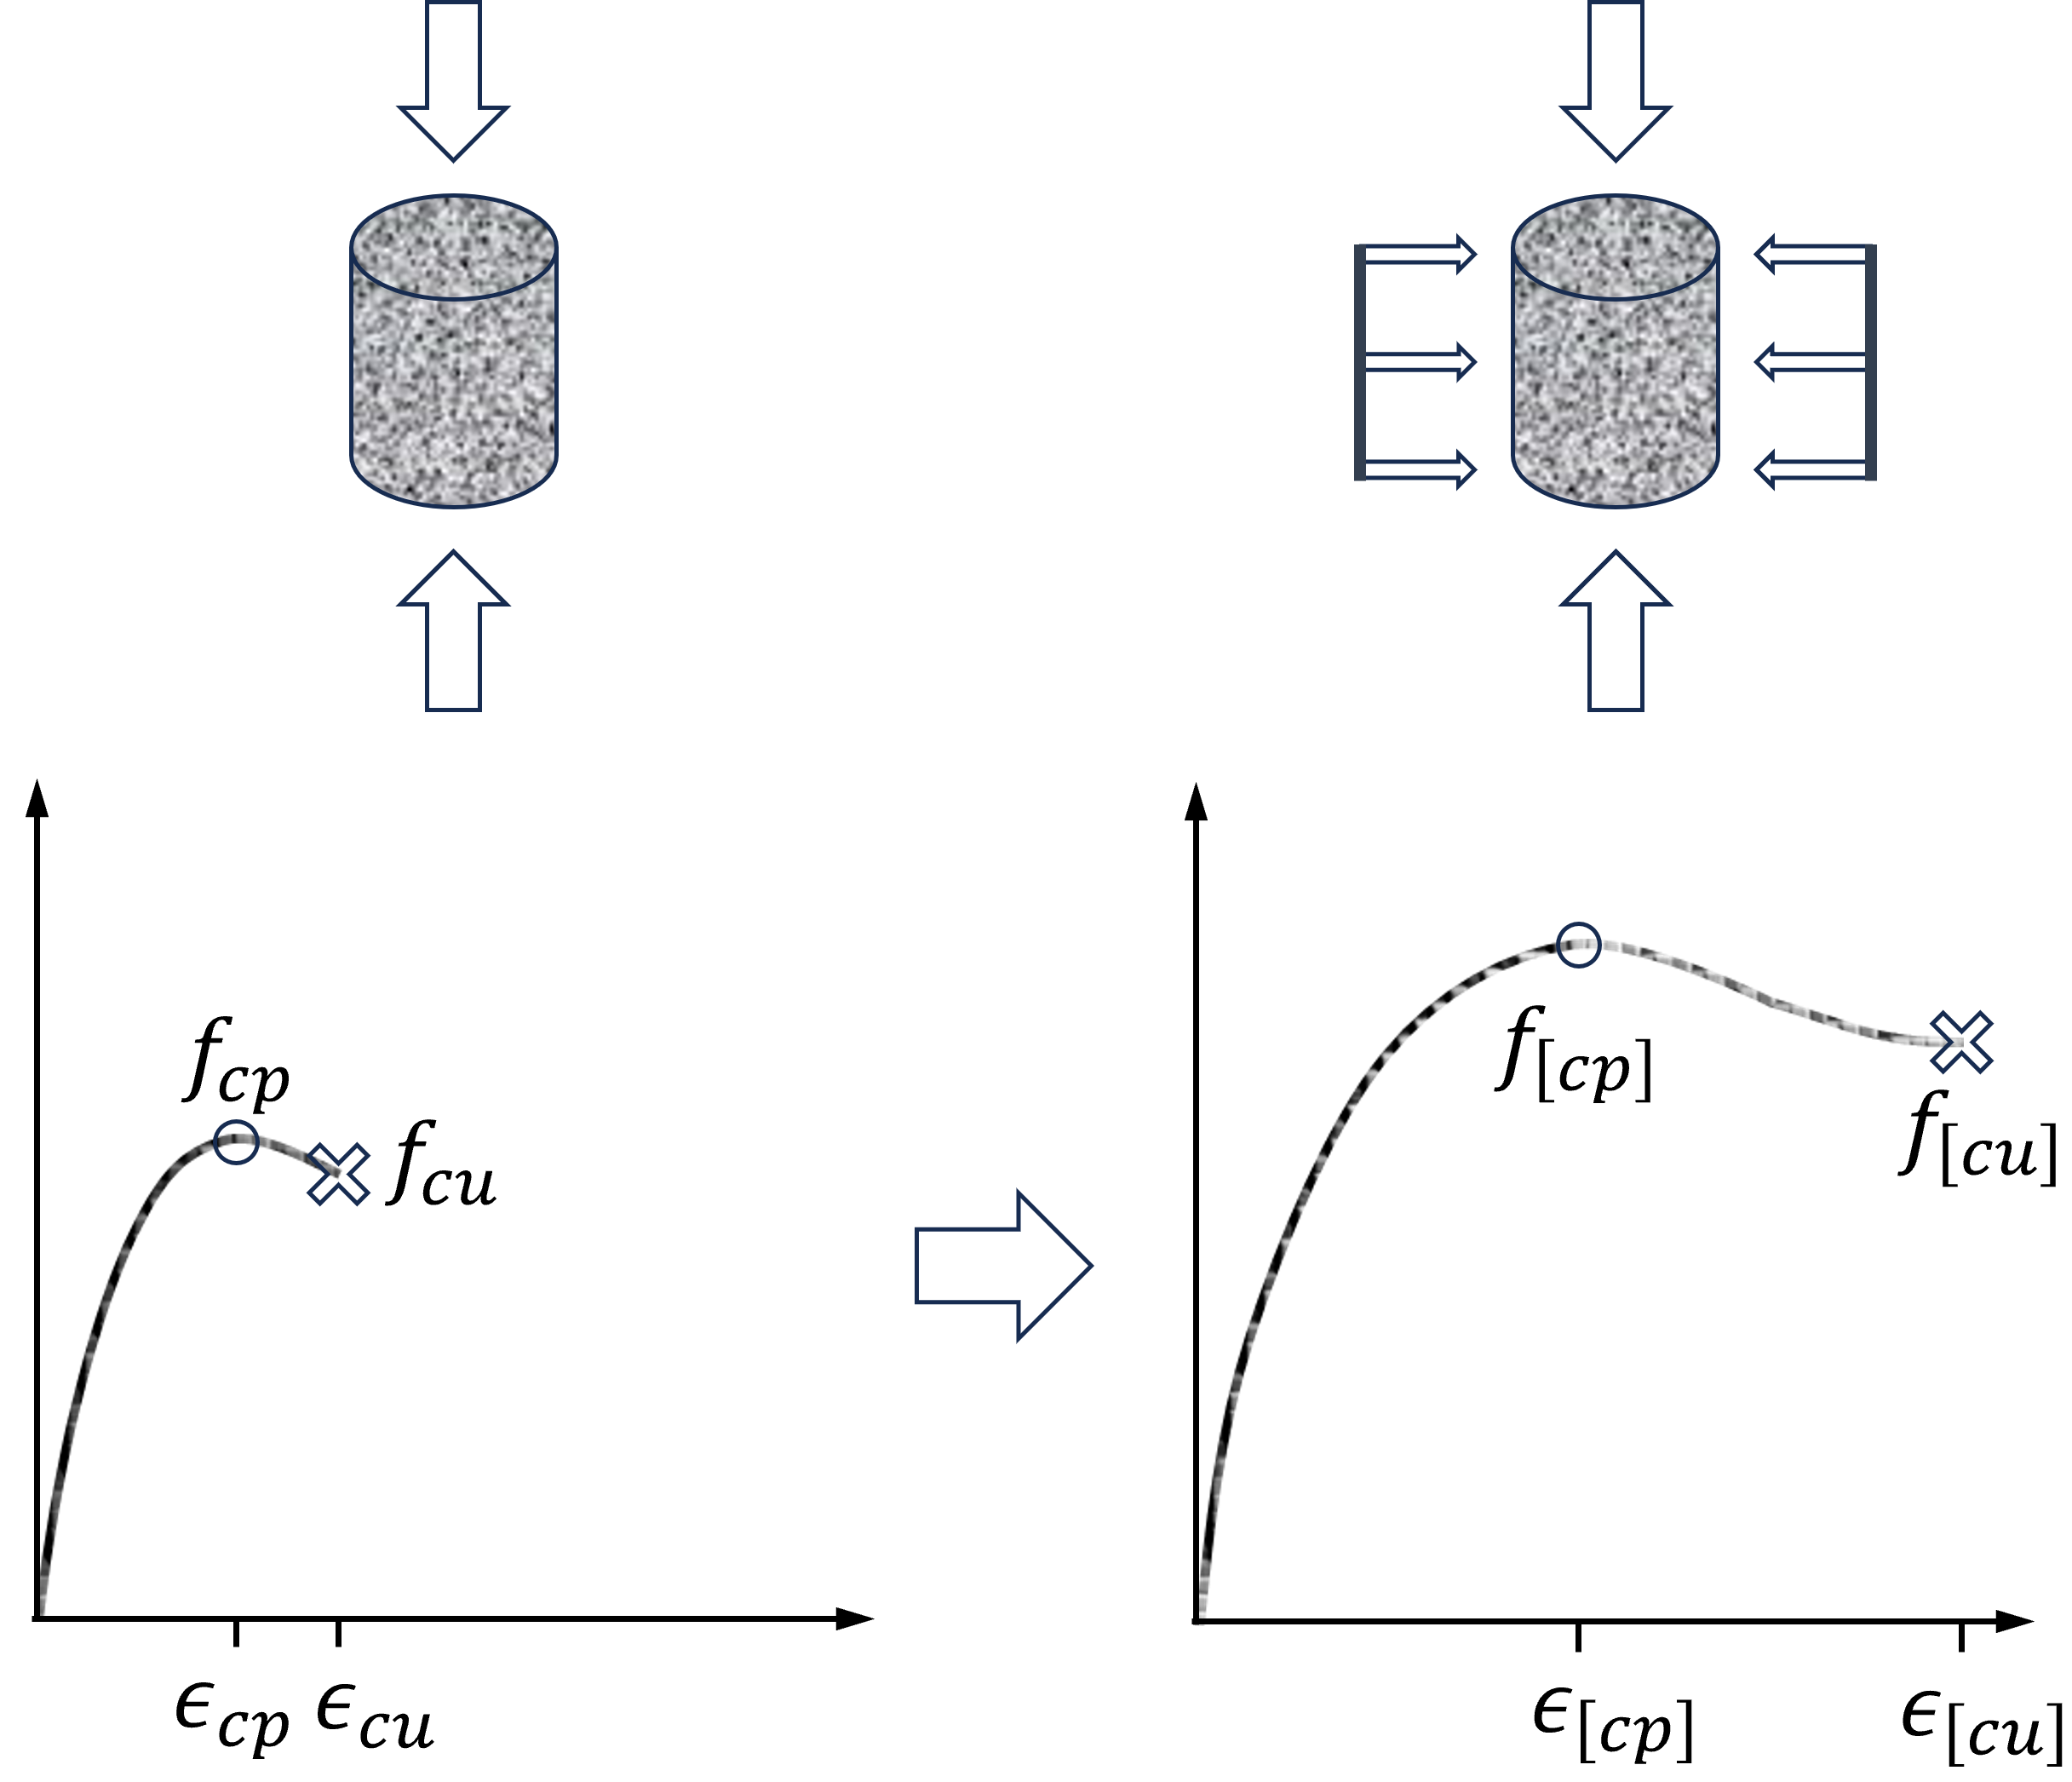
\includegraphics[width=0.6\textwidth]{Part II/figures/confinement.png}
    \caption{Modeling confined concrete often requires an empirical transformation of the unconfined concrete behavior.}
    \label{fig:confined-curve}
\end{figure}

\subsubsection*{In-span Hinges}
In-span hinges are modeled as rotational releases in the superstructure. The translational behavior of in-span hinges are modeled as nonlinear force-displacement relationships, incorporating the effects of pounding, restrainers, bearings, and shear keys. Varying levels of simplification for the hinge models can be employed to linearize or remove discontinuities in the force-displacement relationships.

\subsubsection*{Abutments}
%
%%%%The following equations are provided by \textcite{caltrans2019seismic} for the determination of the effective longitudinal stiffness at the abutments:
%%%%\[
%%%%F_{\mathrm{abut}}=w_{\mathrm{abut}}\left(\frac{5.5 h_{\mathrm{abut}}^{2.5}}{1+2.37 h_{\text {abut }}}\right) R_{s k} \quad (\text{kip})
%%%%\]
%%%%\[
%%%%K_{\text {abut }} = w_{\text {abut }}\left(5.5 h_{\text {abut }}+20\right) R_{\text {sk }} \quad (\text{kip/in}).
%%%%\]

%%%%KM%%%%%\hypertarget{pile-modeling}{%
%%%%KM%%%%%\subsubsection{Pile Modeling}\label{sec:m2-substructure}}
%%%%KM%%%%%A simple model of the flexibility and damping of the soil and the foundation may consist of a spring and a dashpot. The spring parameters are obtained as follows \cite{caltrans2019seismic}:
%%%%KM%%%%%\begin{equation}
%%%%KM%%%%%\begin{aligned}
%%%%KM%%%%%& k=\alpha K, \quad K=\chi E_s d, \quad 
%%%%KM%%%%% \chi=\left(\frac{\pi}{2}\right)^{1 / 4}\left(\frac{E_p}{E_s}\right)^{7 / 40} \\
%%%%KM%%%%%& \alpha=1-\frac{3 \pi}{32 \delta}\left(\frac{\rho_p / \rho_s}{1+v}\right)\left(\frac{\omega d}{V_s}\right), \quad 
%%%%KM%%%%%\delta=2\left(\frac{E_p}{E_s}\right)^{-3 / 40}
%%%%KM%%%%%\end{aligned}
%%%%KM%%%%%\end{equation}

%%%%KM%%%%%\noindent where
%%%%KM%%%%%\begin{table}[h!]
%%%%KM%%%%%    \centering
%%%%KM%%%%%\begin{tabular}{ll}
%%%%KM%%%%%$k$ : & dynamic stiffness \\
%%%%KM%%%%%$K$ : & static stiffness \\
%%%%KM%%%%%$\alpha$ : & dynamic modifier \\
%%%%KM%%%%%$E_s, \rho_s$ : & Elastic modulus and density of soil \\
%%%%KM%%%%%$E_p, \rho_p$ : & Elastic modulus and density of pile material \\
%%%%KM%%%%%$v$ : & Poisson's ratio \\
%%%%KM%%%%%$V_s$ : & shear wave velocity \\
%%%%KM%%%%%$d$ : & pile diameter \\
%%%%KM%%%%%$\omega$ : & fundamental frequency of the bridge bent with a fixed base \\
%%%%KM%%%%%\end{tabular}
%%%%KM%%%%%\end{table}

%%%%KM%%%%%\noindent The pile model of \textcite{boulanger1999seismic} may also be used when high-fidelity pile modeling is needed.
%
%%%%\[
%%%%E_p I_p \frac{d^4 y}{d x^4}+P_x \frac{d^2 y}{dx^2} + E_{py} y - W=0
%%%%\]

\subsubsection{Soil-Shaft Interaction\footnote{For more details, the readers are referred to \cite{reza2024, mohammadinumerical}.}}\label{sec:m2-SSI}
%Beyond the simplified model introduced in \cref{sec:m2-substructure}, for higher fidelity, t
The finite element models that consider the interaction between soil and shafts of monitored bridges are developed and implemented, aiming to provide one using the platform with detailed understanding of the dynamics between soil, ground movements, and structural response.
For each bridge of interest, before modeling, the geotechnical data at the site are gathered through the instrumentation of boreholes available near the structure and relevant documents. The data includes the distribution of different soil and rock layers. 
Moreover, some historical data such as the range of groundwater levels are provided by the bridge owner. With the geotechnical data of the site from boreholes and the historical records, the soil-shaft interaction is analyzed with a two-step finite element modeling approach: (1) the site-specific free-field model, and (2) the drilled shaft model.

\paragraph{Free-field modeling}
The three-dimensional free-field nonlinear soil model calculates the displacements as the applied excitation to the inelastic section models for drilled shafts on the bridge. This is modeled as a column segmented with multiple elements. The constitutive behavior of soil is described by a pressure-independent, multi-yield model with the integration of a range of pertinent soil properties. Then, considering the elastoplastic behavior and the hysteretic damping, the shear velocity ($V_s$) measurements of soil layers are utilized for deriving the strength parameters of the model. Furthermore, the implementation of the Lysmer-Kuhlemeyer dashpot \citep{lysmer1969finite} is achieved by a viscous uniaxial material, where the designed dashpot nodes are connected by zero-length elements. 
For the models with bidirectional loading (2-D), the soil column is modeled with standard eight-node brick elements. 
Finally, subjected to the input motion of the earthquake event of interest, the site responses of the models are obtained, where the dynamic displacement histories are specifically utilized as the excitation of the model of the drilled shafts in the second step.

\paragraph{Soil-shaft interaction modeling}
To accurately capture the shafts' response during seismic events, their sections are modeled with the consideration of inelastic behavior. 
The nodes of the shafts are established with three dimensions and six degrees of freedom. The interaction between soil and the shaft is modeled using an array of springs arranged in two distinct directions (the vertical excitation is not considered), where the spring nodes are connected by zero-length elements. 
The constitutive behavior of these springs is specified such that the lateral springs (in the N-S and W-E directions) function as \emph{p-y} springs. The p-y curves reflect the constitutive model of the corresponding soil type, e.g., sandy soil, clay, and weak rock. The key parameters for the hysteretic model of the soil are determined based on the {\em{p-y}} curves, obtained following the methodology proposed by \cite{reese1978field}. 
For modeling the inelastic shaft, the fiber section is selected \cite{matinrad2023asce}, where the Hognestad concrete model of \cite{yassin1994nonlinear} (see \cref{sec:concrete}) and a bilinear model are employed for the concrete and reinforcing bars, respectively. Furthermore, a force-interpolated element, which accounts for nonlinear curvature distribution along the element's length \cite{spacone1992beam}, is adopted in the modeling. Finally, the displacement at the soil end of each spring, computed from the free-field model at the first step, is applied as a multiple-support excitation.

\paragraph{Integrating soil-shaft interaction models with bridge models}
Given that the bridge and the corresponding foundation models are decoupled and developed separately by the structural engineering and geotechnical engineering teams, respectively, the final step is to integrate them into one holistic model. 
In the current implementation of the platform, the soil-shaft interaction models are integrated with the structural model of the bridge itself by connecting the head node of each shaft pile to the bottom node of the corresponding column by enforcing an equal-degree-of-freedom constraint. 
Such implementation is demonstrated in \cref{sec:painter}.


\section{Limit States}

In the limit state analysis, columns are modeled by a 
distributed-inelasticity frame element with fiber discretized sections.
The node at the base is restrained in all degrees of freedom with the
other (top) node connected to the superstructure being free from any constraints. 
A rigid joint offset is inserted at the top of each column to the center of the cap beam.

\begin{figure}[h!]
\centering
% \includegraphics[height=0.3\textheight]{Part II/figures/general/ColumnGeometry.pdf}
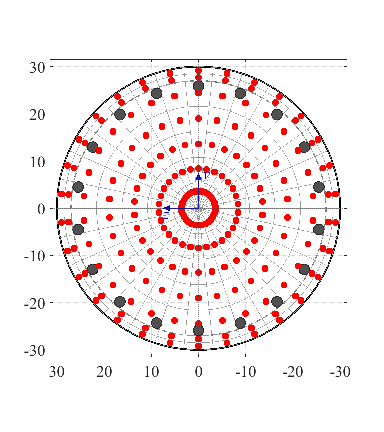
\includegraphics[height=0.3\textheight]{Part II/figures/meloland/Section_Meloland.pdf}
\caption{Strategy of fiber modeling of column members.}
\label{fig:sec_modeling}
\end{figure}

To determine the metric of \emph{damage state} (DS) for a column component given an imposed dynamic loading, maximum strain and maximum displacement are computed from nonlinear response history analysis. 
There are multiple proposed schemes for defining DS, including strain-based DS (\cref{tab:DS}) that models the relationship between fiber strains and component capacity based on previous Caltrans-PEER studies, and ductility-based DS \citep{saini2014probabilistic} that models the relationship between a displacement-based damage index and component capacity. 
The \gls{platform} employs strain-based DS.
\begin{table}[h!]
\centering
\caption{Damage state criteria for strain-based component capacity model.}
\begin{adjustbox}{width=1\textwidth}
\begin{tabular}{@{}cNNLLc@{}}\toprule
\multirow{3}{*}{Label} & \multirow{3}{*}{Description} & \multirow{3}{5cm}{\centering Defining Criteria} & \multicolumn{3}{c}{Damage State} \\ \cmidrule{4-6} & & & Fiber Location & Compression or Tension & Strain \\ \midrule
{DS0} & No damage & -- & -- & -- & -- \\ \midrule
{DS1} & EQ-related tight cracking of cover & Cover cracking: the cover surface reaches tensile strength & Any outermost cover fiber & Tension & \gls{et} \\ \midrule
{DS2} & Moderate cracking (mixed orientations) \& minor spalling/flaking & Minor spalling: the cover surface reaches compressive strength & Any outermost cover fiber  & Compression & \gls{esp} \\ \midrule
{DS3} & Open cracking or major spalling (exterior to confinement) & Major spalling: a significant depth of the cover reaches compressive strength & Any cover fiber at 1/2-3/4 of the cover depth & Compression & \gls{esp} \\ \midrule
{DS4} & Exposed core (interior of confinement) & Exposed core: the entire depth of the cover reaches compressive strength & Any innermost cover fiber & Compression & \gls{esp} \\ \midrule
\multirow{2}{*}{{DS5}} & Visible bar buckling; confinement loss or core shedding & Core shedding: the outer surface of the core begins to fail & Any outermost core fiber & Compression & \gls{ecu} \\ \cmidrule{2-6} & Multi-bar rupture or buckling; large drift; or core crushing & Bar rupture: longitudinal bars reach ultimate tensile strength & Any longitudinal bar & Tension & \gls{esu} \\ \midrule
{DS6} & Column collapse (Near-total loss of axial capacity) & Loss of axial capacity: approximately 1/2 of the core fails & All core fibers at 1/4 of the core depth & Compression & \gls{ecu} \\
\bottomrule
\end{tabular}
\end{adjustbox}
\label{tab:DS}
\end{table}

The damage state metric can be used to further extend the decision-making process for operational actions with standard practices by Caltrans' Structures Maintenance and Investigations group, such as those outlined in the ``Caltrans First Responder Bridge Assessment Guide''. 
For example, DS1-2 corresponds to allowing the structure to remain open; DS3-4 corresponds to inspecting the structure while allowing it to remain open; DS5 corresponds to closing the bridge for further inspection, and DS6 corresponds to closing the bridge immediately. The {\em{decision boundaries}} are to be calibrated in the future as more events occur and are analyzed by the \gls{platform}.

\subsection{Interpretation}

Following their execution on the platform, \glspl{predictor-t1} results are processed into metrics. 
%  they assign a little bit of meaning to the results -- for exmample, we might get a certain strain response and say this equals damage state 1, or minor damage -- flexural cracks.
%  we might get a certain max displacement and say this equals some % drift ratio.
%  the interpretation of these is pretty obvious. 
The processed metrics are displayed on the metric cards (\cref{fig:sam_metrics}). As they are results of \glspl{predictor-t1}, they correspond to \emph{simulated} response values. 
When there are multiple predictors, the desired predictor can be selected from the predictor selection region at the bottom of each metric card.

\begin{figure}%[H]
\centering
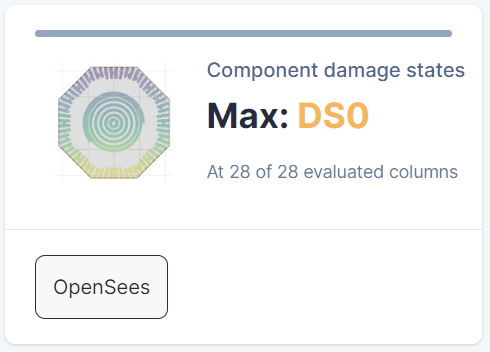
\includegraphics[width=0.5\linewidth]{Part II/figures/predictors/t1_metrics_ds.png}
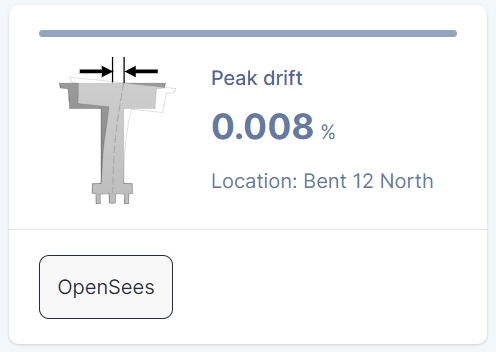
\includegraphics[width=0.5\linewidth]{Part II/figures/predictors/t1_metrics_drift.png}
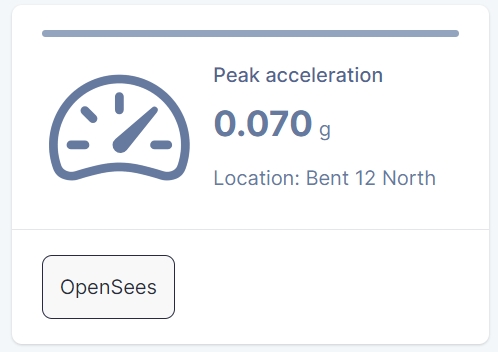
\includegraphics[width=0.5\linewidth]{Part II/figures/predictors/t1_metrics_accel.png}
\caption{Type I predictor metrics.}
\label{fig:sam_metrics}
\end{figure}
